\documentclass[oneside,a4paper]{memoir}
\setsecnumdepth{subsection}

% ABOUT THIS FILE
% ---------------
%
% The goal of this document is to prepare the next (and final?) version of the
% chapter 3.

\usepackage{geometry}
\usepackage{paralist}
\usepackage{hyperref}
\usepackage{amssymb}
\usepackage{amsmath}

\usepackage[T1]{fontenc}
\usepackage[utf8]{inputenc}
\usepackage{inconsolata}

\usepackage[dvipsnames]{xcolor}
\usepackage{xargs}
\usepackage{todonotes}
\newcommandx{\thomasrk}[2][1=]{\todo[linecolor=Plum,backgroundcolor=Plum!25,bordercolor=Plum,#1]{#2}}

\usepackage{mdframed} % or, "mdframed"
\usepackage[amsthm,framed]{ntheorem}

\definecolor{statementline}{HTML}{b7e2d6}

\theoremstyle{break}
\theorembodyfont{\fontshape\rmdefault\selectfont}

\mdfdefinestyle{quoted}{
hidealllines=true,
leftmargin=-15pt,
rightmargin=-15pt,
leftline=true,
innertopmargin=10pt,
innerbottommargin=10pt,
innerrightmargin=15pt,
linewidth=5pt,
linecolor=gray!40,
backgroundcolor=gray!3,
usetwoside=false,
skipabove=\topsep,
skipbelow=\topsep}

\mdfdefinestyle{definition}{
style=quoted,
linecolor=Violet!20,
backgroundcolor=Violet!2}

\mdfdefinestyle{statement}{
style=quoted,
linecolor=PineGreen!30,
backgroundcolor=PineGreen!2}

\newmdtheoremenv[style=definition]{definition}{Definition}[chapter]
\newmdtheoremenv{notation}{Notation}[chapter]
\newmdtheoremenv[style=quoted]{example}{Example}[chapter]
\newmdtheoremenv[style=statement]{corollary}{Corollary}[chapter]
\newmdtheoremenv[style=statement]{lemma}{Lemma}[chapter]
\newmdtheoremenv[style=statement]{theorem}{Theorem}[chapter]

\usepackage{tikz}
\usetikzlibrary{shapes.geometric, positioning, arrows, intersections, fit,
  matrix, shapes, shapes.symbols}

\usepackage{acro}
\DeclareAcronym{cpu}{
  short = CPU,
  long  = Central Processing Unit,
  class = abbrev
}
\DeclareAcronym{mmu}{
  short = MMU,
  long  = Memory Management Unit,
  class = abbrev
}
\DeclareAcronym{bios}{
  short = BIOS,
  long  = Basic Input/Output System,
  class = abbrev
}
\DeclareAcronym{smm}{
  short = SMM,
  long  = System Management Mode,
  class = abbrev
}
\DeclareAcronym{smi}{
  short = SMI,
  long  = System Management Interrupt,
  class = abbrev
}
\DeclareAcronym{apic}{
  short = APIC,
  long  = Advanced Programmable Interrupt Controller,
  class = abbrev
}
\DeclareAcronym{tcb}{
  short = TCB,
  long  = Trusted Computing Base,
  class = abbrev
}


\begin{document}
\chapter{State of the Art of Formal Verification}

% Formal verification consists in proving the correctness of a system,
% characterized by a mathematical model, with respect to certain properties,
% defined as logic formula.
%%
% The result of decades of academic researches and industrial investments is a
% large collection of complementary
% formalisms\,\cite{berthomieu1991petri,mcmillan1989compositional,baeten2005processalgebra,emmi2008interfaceautomata,hoare1969hoare,reynolds2002separation}
% to model systems and defined properties of interest, and
% tools\,\cite{cuoq2012framac,coq,cimatti2002nusmv,jackson2012alloy} to assist
% and automate the verification process.
%%
% This allowed for applying formal verification to a broad variety of computer
% science domains, including cryptographic
% protocols\,\cite{goubault2000crypto,meadows2003crypto},
% compilers\,\cite{leroy2012compcert}, system software
% component\,\cite{klein2009sel4,gu2016certikos} or hardware
% designs\,\cite{lie2003xom,kaivola2009formalintel,reid2016armv8}.
%%
% With regard to \ac{hse} mechanisms, they fall between two domains that are
% hardware design verification and low-level software components verification.
%%
% On the one hand, hardware designs verification often focus on properties
% transparent to the executed software components (\emph{e.g.} cache
% coherency\,\cite{stern1995cachecoherence}, linearizability of SGX
% instructions\,\cite{leslie2015sgx}, hardware-based memory
% isolation\,\cite{lie2003xom}).
%%
% Security gap in interactions of multiple platform components are less subject
% to formal verification, due to their increasing
% complexity\,\cite{potlapally2011hardwaresecurity}.
%%
% Yet they are responsible for architectural attacks we want to avoid.
%%
% On the other hand, low-level software components such as
% seL4\,\cite{klein2009sel4} or CertiKOS\,\cite{gu2016certikos} use the features
% exposed by these components, and are verified against \emph{ad hoc} hardware
% models, whose scope is often limited to necessary hardware features.
%%
%% For our part, we would rather characterize a set of sufficient requirements
%% over low-level software components, such that any software implementation
%% which satisfy these requirements and is executed by the hardware architecture
%% proves to be correct with respect to a targeted property.
%%
% We steer a middle course between these approaches.
%%
% For our part, we would rather characterize sets of requirements over low-level
% software components, such that satisfying these requirements is sufficient to
% ensure the hardware architecture enforces a certain property.
%%
% As a first step, we can verify the correctness of these requirements against a
% hardware model.
%%
% The long term goal of this approach is to focus the verification of low-level
% software components on proving they satisfy these requirements.
%%
% As such, our approach relates to previous research works such as
% RockSalt\,\cite{morrisett2012rocksalt} (validation of arbitrary programs
% against a verified software-based fault isolation\,\cite{wahbe1994sfi} policy)
% or Moat\,\cite{sinha2015moat} (verification of SGX
% enclave\,\cite{costan2016sgxexplained} programs with respect to
% confidentiality).
%
% The rest of this Chapter proceeds as follow.
%%
% First, we give an opinionated introduction to the formal verification of
% hardware and software components with respect to security properties, with
% respect to our objectives (Section~\ref{?}).
%%
% Then, we give a review of several industrial and academic projects which
% implements these approaches (Section~\ref{?}).
%%
% Finally,

Formal verification consists in proving the correctness of a system ---the
\emph{Implementation}--- with respect to certain properties.
%
To that end, a verifier
%
\begin{inparaenum}[(1)]
\item defines a formal description of the system ---the \emph{Specification}---,
  %
\item exhibits a proof that a formal description of the system satisfies a
  statement (defined in an arbitrary logic) which encodes the property with
  respect to which the correctness shall be proven, and
  %
\item exhibits a proof of correspondence between the implementation and the
  specification.
\end{inparaenum}
%
In this context, the terms ``implementation'' and ``specification'' refer to a
subjective relation between two layers of abstraction: the specification is more
abstract than its implementation, and formal verification proofs can be
organized in an arbitrary number of abstraction layers
%
The definition of a specification shall ease the construction of the proof of
correctness, while the correspondence proof allows for extending the properties
of the specification to the implementation.
%
The instantiation of the terms ``formal description'', ``correspondence proof'',
``properties'' or ``correctness proof'' may considerably vary from one system to
another.
%
Similarly, the nature of the proofs and their construction greatly depend on the
tools used by the verifier.
%
For our part, we want to construct correctness proofs of a hardware architecture
specification, with respect to security properties, and using the Coq theorem
prover (as explained in Chapter~\ref{chap:introduction}).
%
The rest of this Chapter is organized with this objective in mind

First, we describe popular formalisms used to define formal descriptions of
hardware specifications (Section~\ref{sec:sota:formalisms}).
%
Then, we focus on the encoding of security properties as logic statements
(Section~\ref{sec:sota:security}).
%
Finally, we give an overview of related works
(Section~\ref{sec:sota:relatedwork}).
% and we conclude this Chapter by positioning our contributions in that respect
% (Section~\ref{...}).

\section{Transition Systems}
\label{sec:sota:formalisms}

The formal verification of discrete systems, such as computing systems, commonly
rely on some sort of \emph{transition systems} to describe the behavior of the
target.
%
More precisely, the system is characterized by a set of \emph{states} and by a
set of \emph{atomic} state-transformation, called \emph{transitions}.
%
Transitions occur when the system interacts with its environment (\emph{e.g.} a
hardware circuit receives a clock signal, a hardware controller receives a
message from a bus, an operating system handles a syscall).
%
Additionally, \emph{labeled} transition systems distinguish between classes of
transitions \emph{via} the use of labels (\emph{e.g.} one label per syscall).

To the best of our knowledge, the more straightforward definition of a labeled
transition system, as used by Vijayaraghavan \emph{et al.} in their work on
modular verification of multiprocessor hardware
designs\,\cite{vijayaraghavan2015modular}, is a tuple
\( \langle S, L, R \rangle \), such that \( S \) is a set of states, \( L \) is
a set of labels, and \( R \subseteq S \times L \times S \) is the transition
relation.

\begin{example}[Airlock System]
  Figure~\ref{fig:sota:airlock-lts} illustrates an instantiation of this
  definition for a simple airlock system.
  %
  An airlock system is a device made of two doors, and an intermediary chamber.
  %
  To get across a airlock system, a user requests the opening of the first door,
  enters the chamber, waits for the system to close the first door and open the
  second door, and exits the chamber.

  \begin{itemize}
  \item A door of the system can be either \( \mathtt{open} \) or
    \( \mathtt{close} \).
    %
    The set of states of the airlock system reflects the combinatronics of the
    doors states.
  \item A transition is characterized by the opening (\( \mathtt{Open}_i\), with
    \( i \in \{1, 2\} \)) and closing (\( \mathtt{Close}_i \), with
    \( i \in \{1, 2\} \)) of a door of the system.
    %
  \item The system does not allow the simultaneous opening of both doors, as
    stated by the definition of \( R \) which does not contains a transition
    which leads to the state \( (\mathtt{open}, \mathtt{open}) \).
  \end{itemize}
\end{example}

\begin{figure}
  \begin{center}
    % the mathematical definition
    \begin{minipage}[c]{0.55\linewidth}
      \[
        \begin{array}{rcl}
          S & \triangleq & \{ \mathtt{open}, \mathtt{close} \}^2 \\
          L & \triangleq & \{ \mathtt{Open}_1, \mathtt{Close}_1, \mathtt{Open}_2,
                           \mathtt{Close}_2 \} \\
          R & \triangleq & \{ (\mathtt{close}, \mathtt{close}), \mathtt{Open_1},
                           (\mathtt{open}, \mathtt{close}), \\
            & & \ (\mathtt{close}, \mathtt{close}), \mathtt{Open_2},
                (\mathtt{close}, \mathtt{open}), \\
            & & \ (\mathtt{open}, \mathtt{close}), \mathtt{Close_1},
                (\mathtt{close}, \mathtt{close}), \\
            & & \ (\mathtt{close}, \mathtt{open}), \mathtt{Close_2},
                (\mathtt{close}, \mathtt{close}) \}
        \end{array}
      \]
    \end{minipage}
    \hfill
    % a tikzpicture to illustrate the resulting automata
    \begin{minipage}[c]{0.40\linewidth}
      \begin{center}
        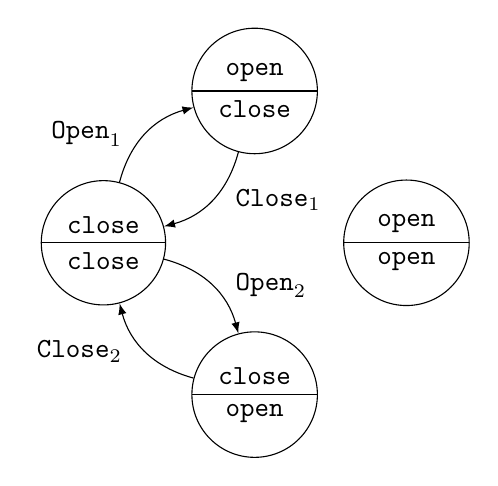
\begin{tikzpicture}
          \node [draw, circle split, text width=30pt, text badly centered] (cc)
          {\( \mathtt{close} \) \nodepart{lower} \( \mathtt{close} \)};%
          \node [right=of cc] (x) {};%
          \node [draw, circle split, above=of x, text width=30pt, text badly
          centered] (oc) {\( \mathtt{open} \) \nodepart{lower}
            \( \mathtt{close} \)};%
          \node [draw, circle split, below=of x, text width=30pt, text badly
          centered] (co) {\( \mathtt{close} \) \nodepart{lower}
            \( \mathtt{open} \)};%
          \node [draw, circle split, right=of x, text width=30pt, text badly
          centered] (oo) {\( \mathtt{open} \) \nodepart{lower}
            \( \mathtt{open} \)};%

          \draw [-latex] (cc) edge [bend left] node [xshift=-5pt, left]
          {\( \mathtt{Open}_1 \)} (oc);%
          \draw [-latex] (oc) edge [bend left] node [xshift=5pt, right]
          {\( \mathtt{Close}_1 \)} (cc);%

          \draw [-latex] (cc) edge [bend left] node [xshift=5pt, right]
          {\( \mathtt{Open}_2 \)} (co);%
          \draw [-latex] (co) edge [bend left] node [xshift=-5pt, left]
          {\( \mathtt{Close}_2 \)} (cc);%

        \end{tikzpicture}
      \end{center}
    \end{minipage}

    \caption{An simple airlock system modeled as a labeled transition system}
    \label{fig:sota:airlock-lts}
  \end{center}
\end{figure}

There are many modeling structures one can use to characterize transition
systems, with each variant better suited to tackle a particular class of
systems.
%
For instance, the Kripke structure\,\cite{kripke1971semantical} is a notorious
variation of (labeled) transition systems used in model
checking\,\cite{clarke1999model}, while Petri net\,\cite{peterson1981petri},
process algebra\,\cite{bergstra1984process} or interface
automata\,\cite{de2001interface} are better suited to model concurrent systems.

\subsection{Operational Semantics}

\subsection{Denotational Semantics}

\subsection{Compositional Modeling}

\section{Specifying Security Policies}
\label{sec:sota:security}

\section{A Tour of Large Verified Systems}
\label{sec:sota:relatedwork}

\subsection{Hardware Systems}

\paragraph{Intel.}

\paragraph{ARM.}

\paragraph{XOM.}

\bibliographystyle{unsrt}%
\bibliography{manuscript}
\end{document}